\documentclass[11pt,a4paper,twocolumn]{article}
\usepackage[utf8]{inputenc}
\usepackage{amsmath}
\usepackage{graphicx}
\usepackage{hyperref}
\usepackage{setspace}
\usepackage{enumerate}
\title{Assignment7}
\author{Aravind A Anil}
\date{\today}
\begin{document}
\maketitle
\textbf{Problem Statement:(6.17):}A person plays a game of tossing a coin thrice.For each head,he is given Rs 2 by the organiser of the game and for each tail,he has to give Rs 1.50 to the organiser.Let X denotes the amount gained or lost by the person.show that X is random variable and exhibit it as a function on the sample space of the experiment.\\
\textbf{Solution:},here we are tossing a coin three times so,\\
.Let $X_i,i=0,1,2,$ be the value at the end of each toss.\\Then $X_i=X_{i-1}+Y$,Where $Y\in\{2,-1.5\}$ 
$X_{0}=Y$\\
$X_{1}=X_{0}+Y$\\
$X_{2}=X_{1}+Y$\\
$Z\in{0,1}$,where 0 represent getting a tail and 1 represents getting a head
\begin{table}[ht]
    \centering
    \begin{tabular}{|c|c|c|}
\hline
     &head&tail  \\
     \hline
     Z&1&0\\
     \hline
\end{tabular}
\end{table}
\begin{enumerate}
  \item \textbf{$X_{0}$ can have two values}
  \begin{enumerate}
      \item Case-\romannumeral1
    \begin{itemize}
    \item When \textbf{Z=0},\\
    $X_{0}=-1.5$\\
$Pr(X_{0}|Z=0)=\frac{1}{2}$
    \end{itemize}
      \item Case-\romannumeral2
\begin{itemize}
    \item When \textbf{Z=1},\\
    $X_{0}=2$\\
    $Pr(X_{0}|Z=1)=\frac{1}{2}$
\end{itemize}
  \end{enumerate}
\newpage
    \item{\textbf{$X_{1}$ can have four values}}
    \begin{enumerate}
        \item Case-\romannumeral1
        \begin{itemize}
        \item When $X_{0}=-1.5$ \& $Z=0$\\
        \end{itemize}
        \begin{align*}
         X_{1}&=-1.5-1.5\\
         &=-3
        \end{align*}
        \begin{align*}
        \hspace{-2cm}
          Pr(X_{1}|Z=0,X_{0}=-1.5)&=\frac{1}{2}\times\frac{1}{2}\\
        &=\frac{1}{4}
        \end{align*}
        \item Case-\romannumeral2
        \begin{itemize}
          \item When $X_{0}=2 \& Z=0$
        \end{itemize}
        \begin{align*}
         X_{1}&=2-1.5\\
         &=.5
         \end{align*}
          \begin{align*}
        \hspace{-2cm}
          Pr(X_{1}|Z=0,X_{0}=2)&=\frac{1}{2}\times\frac{1}{2}\\
        &=\frac{1}{4}
        \end{align*}
       \item Case-\romannumeral3
       \begin{itemize}
           \item When $X_{0}=-1.5$\& $Z=1$
           \begin{align*}
         X_{1}&=-1.5+2\\
         &=.5
         \end{align*}
         \begin{align*}
        \hspace{-2cm}
          Pr(X_{1}|Z=1,X_{0}=-1.5)&=\frac{1}{2}\times\frac{1}{2}\\
        &=\frac{1}{4}
        \end{align*}
       \end{itemize}
         \item Case-\romannumeral4
         \begin{itemize}
             \item  When $X_{0}=2$\& $Z=1$
             \begin{align*}
         X_{1}&=2+2\\
         &=4
         \end{align*}
         \begin{align*}
        \hspace{-2cm}
          Pr(X_{1}|Z=1,X_{0}=2)&=\frac{1}{2}\times\frac{1}{2}\\
        &=\frac{1}{4}
        \end{align*}
         \end{itemize}
    \end{enumerate}
    \item \textbf{$X_{2}$ can have eight values}
    \begin{enumerate}
        \item Case-\romannumeral1
\begin{itemize}
    \item When $X_{1}=-3$ \& $Z=0$
    \begin{align*}
        X_{2}&=-3-1.5\\
        &=-4.5
    \end{align*}
    \begin{align*}
    \hspace{-2.5cm}
        Pr(X_{2}|X_{1}=-3,Z=0)&=\frac{1}{4}\times\frac{1}{2}\\
        &=\frac{1}{8}
    \end{align*}
\end{itemize}
        \item Case-\romannumeral2
      \begin{itemize}
      \item When $X_{1}=-3$ \& $Z=1$
    \begin{align*}
        X_{2}&=-3+2\\
        &=-1
    \end{align*}
    \begin{align*}
    \hspace{-2.5cm}
        Pr(X_{2}|X_{1}=-3,Z=1)&=\frac{1}{4}\times\frac{1}{2}\\
        &=\frac{1}{8}
    \end{align*}
    \end{itemize}
        \item Case-\romannumeral3
        \begin{itemize}
          \item When $X_{1}=.5$ \& $Z=0$
    \begin{align*}
        X_{2}&=.5+-1.5\\
        &=-1
    \end{align*}
    \begin{align*}
    \hspace{-2.5cm}
        Pr(X_{2}|X_{1}=.5,Z=0)&=\frac{1}{4}\times\frac{1}{2}\\
        &=\frac{1}{8}
    \end{align*}
        \end{itemize}
        \item Case-\romannumeral4
    \begin{itemize}
        \item When $X_{1}=.5$ \& $Z=1$
    \begin{align*}
        X_{2}&=.5+2\\
        &=2.5
    \end{align*}
    \begin{align*}
    \hspace{-2.5cm}
        Pr(X_{2}|X_{1}=.5,Z=1)&=\frac{1}{4}\times\frac{1}{2}\\
        &=\frac{1}{8}
    \end{align*}
    \end{itemize}
    \item Case-\romannumeral5\\
    Case-$\romannumeral5$ will be same as Case-$\romannumeral3$ since $X_{1}=.5$ is occuring two times\\
    \begin{align*}
         X_2&=.5-1.5\\
         &=-1
    \end{align*}
    $Pr(X_{2}|X_{1}=.5,Z=0)=\frac{1}{8}$\\
     \item Case-\romannumeral6\\
    Case-$\romannumeral6$ will be same as Case-$\romannumeral4$ since $X_{1}=.5$ is occuring two times\\
    \begin{align*}
         X_2&=.5+2\\
         &=2.5
    \end{align*}
    $Pr(X_{2}|X_{1}=.5,Z=1)=\frac{1}{8}$\\
    \item Case-\romannumeral7
    \begin{itemize}
        \item When $X_{1}=4$ \& $Z=0$
    \begin{align*}
        X_{2}&=4-1.5\\
        &=2.5
    \end{align*}
    \begin{align*}
        \hspace{-2.5cm}
        Pr(X_{2}|X_{1}=4,Z=0)&=\frac{1}{4}\times\frac{1}{2}\\
        &=\frac{1}{8}
    \end{align*}
    \end{itemize}
\newpage
     \item {Case-$\romannumeral8$}
     \begin{itemize}
         \item When $X_{1}=4$ \& $Z=0$
    \begin{align*}
        X_{2}&=4+2\\
        &=6
    \end{align*}
    \begin{align*}
        \hspace{-2.5cm}
        Pr(X_{2}|X_{1}=4,Z=1)&=\frac{1}{4}\times\frac{1}{2}\\
        &=\frac{1}{8}
    \end{align*}
    \end{itemize}
    \end{enumerate}
\end{enumerate}
Here values of $X_{2}$ can be 6,2.5,-1,-4.5\\
All these are real values\\
Hence,\textbf{$X_{2}$=\{6,2.5,-1,-4.5\}}\\
\& $X_2$ is a \textbf{Random Variable}
\begin{table}[h!]
    \centering
    \begin{tabular}{|c|c|c|c|c|}
    \hline
         $X_{2}$&-4.5&-1&2.5&6  \\
         \hline
         $Pr(X_{2})$&$\frac{1}{8}$&$\frac{3}{8}$&$\frac{3}{8}$&$\frac{1}{8}$\\
         \hline
    \end{tabular}
    \caption{Probability Distribution of $X_{2}$}
    \label{tab:my_label}
\end{table}
\newpage
\begin{figure}[h!]
    \centering
    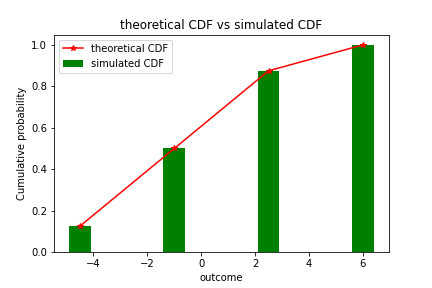
\includegraphics[width=9cm]{cdf.png}
    \caption{CDF}
\end{figure}
\begin{figure}[h!]
    \centering
    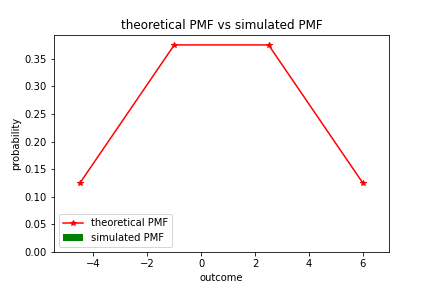
\includegraphics[width=9cm]{pmf.png}
    \caption{PMF}
\end{figure}
\end{document}
